% Section V -- Results and Discussion
% Draft 1 (22 Nov 2026). Numbers from results/ (round 2, Octave + HiGHS run of model/main.m); re-check
% against the MATLAB run before submission. Figures from tools/make_results_figs.py.
\section{Results and Discussion}
\label{sec:results}

\subsection{Optimal Configuration}
Table~\ref{tab:base} compares the optimal micro-grid with the reference supply for the base load,
the measured feeder availability and a tilt of 30$^\circ$, which is the cheapest of the four tilts
studied; 40$^\circ$ costs \$174/yr (0.06\%) more. The optimum combines 976~kWp of PV with a
2,623~kWh / 786~kW battery and needs no more than 354~kW of the existing diesel plant, against
519~kW in the reference. PV supplies 72.6\% of the load directly or through the battery, diesel
energy falls from 977 to 168~MWh/yr, and grid purchases fall from 480 to 295~MWh/yr. The annualized
cost drops from \$498,890 to \$299,859 per year, a saving of \$199,031/yr (39.9\%), and the LCOE
from 0.342 to 0.206~\$/kWh. All load, critical and non-critical, is served in every hour.

\begin{table}[!t]
\centering
\caption{Base-Case Micro-Grid Against the Reference Supply}
\label{tab:base}
\footnotesize
\setlength{\tabcolsep}{4pt}
\begin{tabular}{@{}l r r@{}}
\toprule
 & Reference & Micro-grid \\
\midrule
PV (kWp)                         & --      & 976 \\
Battery (kWh / kW)               & --      & 2,623 / 786 \\
Diesel capacity used (kW)        & 519     & 354 \\
Grid energy (MWh/yr)             & 480     & 295 \\
Diesel energy (MWh/yr)           & 977     & 168 \\
Fuel (L/yr)                      & 252,947 & 43,392 \\
Renewable fraction               & 0\%     & 72.6\% \\
PV curtailed                     & --      & 29.0\% \\
Battery cycles (per yr)          & --      & 217 \\
Annualized cost (\$/yr)          & 498,890 & 299,859 \\
\quad without throughput cost    & 498,890 & 288,466 \\
LCOE (\$/kWh)                    & 0.342   & 0.206 \\
CO$_2$ (t/yr)                    & 1,014   & 323 \\
Unserved load                    & 0       & 0 \\
\bottomrule
\end{tabular}
\end{table}

Of the annualized cost of the micro-grid, 38\% is capital recovery of the PV and battery, 20\% is fuel,
27\% is grid energy, and the remainder is operation and maintenance. Because the battery capital cost
is spread over its 15-year calendar life and each discharged kWh is also charged
0.020~\$/kWh~\cite{seger2023}, battery wear is counted twice in the objective. Removing the throughput
term lowers the cost to \$288,466/yr (a 42.2\% saving); the term is kept in the optimization because it
prevents needless cycling, so the reported savings are conservative. At 217 cycles per year the cells
reach about 3,260 cycles in 15 years, well below their cycle life, so calendar ageing rather than
cycling sets the replacement date.

\subsection{Operation and Seasonal Behaviour}
Fig.~\ref{fig:dispatch} shows the dispatch in the week of the highest load and in a summer week. In
winter the PV output covers only part of the daytime load, the battery is charged while the feeder is
energized, and the diesel carries most of the hours without grid supply on the busy ski days, when the
lifts, chalets and restaurants peak together. In summer the PV charges the
battery by midday, the battery carries the evening and night, and the diesel is almost idle.

\begin{figure}[!t]
\centering
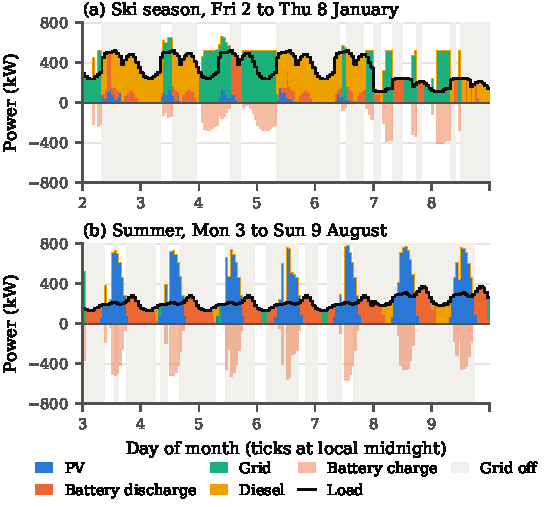
\includegraphics[width=\columnwidth]{figs/res_dispatch_weeks.pdf}
\caption{Hourly dispatch of the base case in (a) the week of the highest load and (b) a summer week.
Sources are stacked above zero and battery charging is drawn below it; shading marks hours without
grid supply.}
\label{fig:dispatch}
\end{figure}

The monthly balance in Fig.~\ref{fig:monthly} shows the seasonal mismatch that drives the design.
December to March holds 46\% of the annual load but only 22\% of the available PV energy. In those
months the PV output is almost fully used (90\%), and they account for 87\% of the diesel energy and
88\% of the grid purchases. From April to November the PV exceeds the demand, and 93\% of the
curtailed energy falls in those months, mostly in the low-load spring and early summer. Winter is
therefore the binding season: the PV array is sized for the winter months, and its summer surplus has
no use in the base case. This surplus is what grid export would monetize (Section~\ref{sec:export}).

\begin{figure}[!t]
\centering
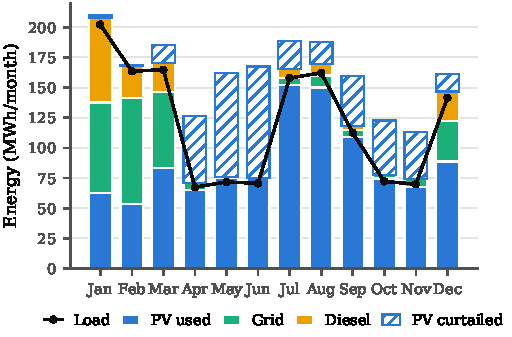
\includegraphics[width=\columnwidth]{figs/res_monthly_energy.pdf}
\caption{Monthly energy supplied by source in the base case, with the PV energy that is curtailed and
the monthly load.}
\label{fig:monthly}
\end{figure}

\subsection{Reliability and the No-Shedding Base Case}
When the model is allowed to shed non-critical load, it places the shedding in the ski season
(Table~\ref{tab:lpsp}). With a 1\% limit, 92\% of the shed energy falls on ski days and 48\% within a
single week in January, with up to 266~kW shed at once against a 519~kW peak. The reason is
structural: each shed kWh saves the same diesel cost whatever the hour, so the timing is a tie in
cost, and the model resolves it at the diesel peaks, which are the ski peaks. Shedding is therefore
concentrated exactly when the club earns its revenue, while the whole 1\% allowance is worth only
\$5,508/yr. Prohibiting shedding on ski days gives the same saving and moves the shedding to
non-ski days. The PV and battery sizes do not change between LPSP 0 and 5\%;
shedding only lowers the diesel capacity that is used, from 354 to 94~kW, and the generators already
exist. The base case therefore requires that no load is shed.

\begin{table}[!t]
\centering
\caption{Where Load Is Shed When It Is Allowed}
\label{tab:lpsp}
\footnotesize
\setlength{\tabcolsep}{3pt}
\begin{tabular}{@{}l r r r r r@{}}
\toprule
LPSP & Shed & Hours & On ski & Diesel & Saving \\
limit & (MWh) & & days & (kW) & (\$/yr) \\
\midrule
0 (base)            & 0    & 0   & --   & 354 & -- \\
0.5\%               & 7.3  & 56  & 96\% & 268 & 2,754 \\
1\%                 & 14.6 & 117 & 92\% & 233 & 5,508 \\
2\%                 & 29.1 & 178 & 92\% & 187 & 11,016 \\
5\%                 & 72.9 & 344 & 89\% & 94  & 27,539 \\
1\%, no ski days & 14.6 & 95  & 0\%  & 354 & 5,508 \\
\bottomrule
\end{tabular}
\end{table}

The design was also checked against the weather of 2014--2023, with the sizes fixed and the dispatch
re-optimized for each year. With the existing diesel plant available, all load is served in every year;
the annualized cost ranges from \$277,378 to \$311,776, at most 4\% above the design year, and the
diesel output reaches 392~kW in the worst year. If the diesel were limited to the 354~kW of the design
year, the worst year (2018) would leave 0.01\% of the load unserved, all of it non-critical. The lift
recovery reserve of 30~kWh adds only \$74/yr.

\subsection{Economic Assessment}
The investment is \$1.235M: \$732k for the PV and \$504k for the battery. The diesel plant is
existing and sunk. Against the reference, the cash operating cost falls by \$325,726 in the first
year, mainly through avoided fuel. Because PV output degrades by 0.7\%/yr, the saving falls to
\$307,595 by year 25. The battery is replaced in year 15 for \$504k, and the remaining life of the
PV and the second battery is credited as a salvage value of \$290k in year 25.
At the base real discount rate of 7.11\%, the NPV is \$2.33M, the real IRR is 25.8\%, and the simple
and discounted paybacks are 3.8 and 4.6 years (Fig.~\ref{fig:finance}a). Because the funder and its
cost of capital are not known, Fig.~\ref{fig:finance}b gives the NPV against the discount rate: it
stays positive at any rate below the IRR, and it is \$1.15M at 12.4\%, the high rate of the
sensitivity analysis. With the low replacement cost of 125~\$/kWh, the NPV rises to \$2.38M.

\begin{figure}[!t]
\centering
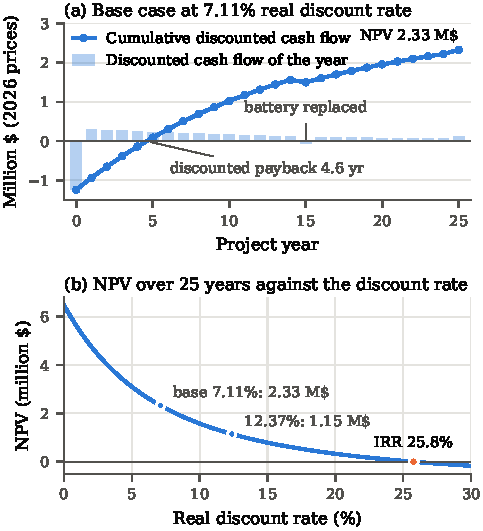
\includegraphics[width=\columnwidth]{figs/res_finance.pdf}
\caption{Finance of the base case: (a) yearly and cumulative discounted cash flow against the
reference supply; (b) NPV over 25 years against the real discount rate.}
\label{fig:finance}
\end{figure}

The payback is much shorter than in the ski-resort studies reviewed in Section~II, which report about
8 and 11 years for PV without storage~\cite{scuderi2025,lewicki2024}. Those resorts have reliable
grids, so PV displaces grid energy at the retail tariff. At Faqra the grid supplies only about 8~h per
day, and the PV and battery mainly displace diesel energy costing about 0.38~\$/kWh at the base fuel
price. Of the reduction in operating cost, 86\% comes from fuel and diesel maintenance and 14\% from
grid energy.

\subsection{Diesel Price}
Fig.~\ref{fig:diesel} repeats the optimization for diesel prices from 0.60 to 2.00~\$/L, which covers
the Lebanese range of 0.80--1.52~\$/L observed in 2023--2026 and extends beyond it. Each point is
compared with a reference at the same price. The NPV is positive at every price, from \$0.42M
(IRR 15.7\%) at 0.60~\$/L to \$3.78M (IRR 34.1\%) at 2.00~\$/L. Within the observed range it lies
between \$0.89M at 0.80~\$/L and about \$2.6M at 1.52~\$/L (interpolated). The optimal system shrinks as the fuel gets cheaper, to 491~kWp
and 726~kWh at 0.60~\$/L. Below about 1.0~\$/L, own diesel generation costs less per kWh than EDL
energy, so the optimal system stops buying grid energy (Fig.~\ref{fig:diesel}b). At 0.99~\$/L the
diesel fuel and maintenance cost per kWh at full load equals the tariff.

\begin{figure}[!t]
\centering
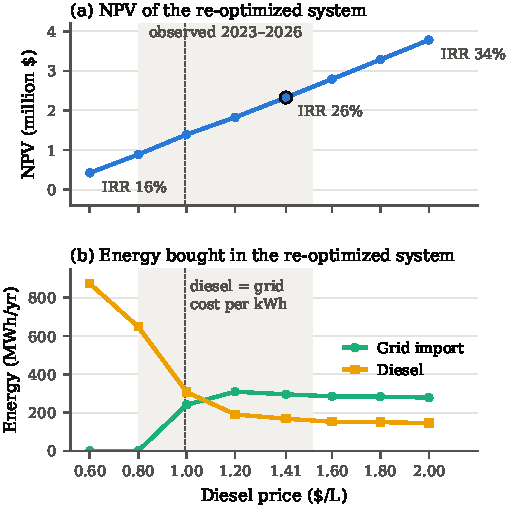
\includegraphics[width=\columnwidth]{figs/res_diesel_sweep.pdf}
\caption{Diesel price sweep with sizes re-optimized at each price: (a) NPV, with the IRR at three
prices; (b) grid and diesel energy. The shaded band is the range observed in 2023--2026, and the
dashed line is the price at which diesel and grid energy cost the same per kWh.}
\label{fig:diesel}
\end{figure}

\subsection{Grid Export}
\label{sec:export}
Lebanon's 2023 law on distributed renewable energy allows net metering and peer-to-peer sales, but the
credit terms have not been set, so export is assessed only as a sensitivity (Table~\ref{tab:export}).
Under net metering at the tariff, capped at the year's import, the optimal PV grows by 153~kWp,
curtailment falls from 29.0 to 21.5\%, and the 301~MWh exported offsets the whole grid bill. The
saving then rises to 54.2\% and the NPV to \$3.10M. When export is sold at a fixed price without a
cap, the saving rises from 42.2\% at 0.05~\$/kWh to 56.1\% at 0.27~\$/kWh. Export is possible only
while the feeder is energized, which limits it to about a third of the hours. Even a low export price
therefore adds value, but the base-case conclusion does not depend on it.

\begin{table}[!t]
\centering
\caption{Grid Export Cases (Sizes Re-Optimized)}
\label{tab:export}
\footnotesize
\setlength{\tabcolsep}{3pt}
\begin{tabular}{@{}l r r r r@{}}
\toprule
Case & Export (MWh) & PV (kWp) & Saving & NPV (\$M) \\
\midrule
No export (base)        & 0   & 976   & 39.9\% & 2.33 \\
Net metering, 0.27 \$/kWh & 301 & 1,129 & 54.2\% & 3.10 \\
Sold at 0.05 \$/kWh     & 256 & 1,098 & 42.2\% & 2.47 \\
Sold at 0.10 \$/kWh     & 288 & 1,199 & 44.9\% & 2.62 \\
Sold at 0.20 \$/kWh     & 327 & 1,344 & 51.1\% & 2.96 \\
Sold at 0.27 \$/kWh     & 374 & 1,465 & 56.1\% & 3.24 \\
\bottomrule
\end{tabular}
\end{table}

\subsection{Sensitivity Analysis}
Fig.~\ref{fig:tornado} summarizes the one-at-a-time sensitivities as the saving against each case's
own reference. Apart from export, the diesel price, the irradiance data set, the discount rate and the
battery cost have the largest effect. The saving remains positive in every case, from 23.7\% at a diesel price of
0.80~\$/L to 56.1\% with export at the tariff. The load scenario hardly changes the relative saving
(40.9--41.1\%), because the sizes scale with the load. The grid availability matters little in
relative terms: with no grid at all the saving is still 40.8\%, because the reference would then also
run entirely on diesel.

\begin{figure}[!t]
\centering
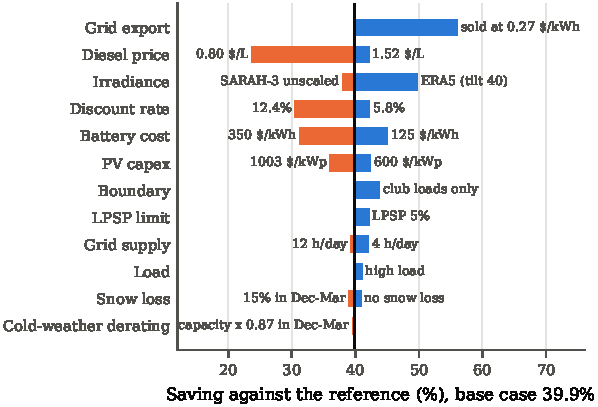
\includegraphics[width=\columnwidth]{figs/res_tornado.pdf}
\caption{Saving against the reference for one-at-a-time changes from the base case. Each case is
re-optimized and compared with a reference under the same assumptions.}
\label{fig:tornado}
\end{figure}

\subsection{Environmental Impact}
The micro-grid cuts fuel use by 83\%, from 252,947 to 43,392~L/yr. Counting the emissions of grid
energy as well, CO$_2$ falls from 1,014 to 323~t/yr, a reduction of 691~t/yr (68\%). Diesel run hours
fall from 5,800 to 776 per year, which also reduces noise, local pollution and fuel deliveries on the
mountain road.

\subsection{Hypotheses Revisited}
\emph{H1, savings come mainly from displaced diesel:} supported. Fuel and diesel maintenance make up
86\% of the operating-cost reduction.
\emph{H2, winter is the binding season:} supported. December to March uses 90\% of its PV, while
93\% of the curtailment falls in the other months, and the diesel and grid energy that remain are
concentrated in winter.
\emph{H3, steep tilts and retained generators:} partly supported. Retaining the generators is
cheaper than eliminating them: even when new diesel capacity must be bought at 750~\$/kW, the
optimum still includes 308~kW. The model does not include the snow-reflection gain at steep tilts, so
the tilt part is not tested. With the irradiance used, 30$^\circ$ is the cheapest tilt and 40$^\circ$
costs 0.06\% more.
\emph{H4, serving critical loads first reduces storage:} not supported. The PV and battery sizes are
the same for LPSP limits from 0 to 5\%; allowing non-critical load to be shed only reduces the diesel
capacity used.

\subsection{Limitations}
The load is reconstructed from benchmarks rather than metered, and the study relies on public data
only, so the results are scenario estimates. The diesel model treats the plant as several sets running
at full-load efficiency; this understates fuel use in both cases, but it understates it more in the
reference, which burns 5.8 times more fuel, so the savings are conservative. Taxes, inflation and the
financing structure are not modelled, and the export terms are not yet regulated.
